\documentclass[11pt, oneside]{article}   	% use "amsart" instead of "article" for AMSLaTeX format
\usepackage{geometry}                		% See geometry.pdf to learn the layout options. There are lots.
\geometry{letterpaper}                   		% ... or a4paper or a5paper or ... 
%\geometry{landscape}                		% Activate for for rotated page geometry
%\usepackage[parfill]{parskip}    		% Activate to begin paragraphs with an empty line rather than an indent
\usepackage{graphicx}				% Use pdf, png, jpg, or eps� with pdflatex; use eps in DVI mode
								% TeX will automatically convert eps --> pdf in pdflatex		
\usepackage{amssymb}
\usepackage{amsmath}
\usepackage{parskip}
\usepackage{color}

\title{Kepler (part 8) Fitzpatrick derivation}
%\author{The Author}
%\section{}
% \subsection*{R code}
\date{}							% Activate to display a given date or no date

\graphicspath{{/Users/telliott_admin/Dropbox/Tex/png/}}

% \begin{center} 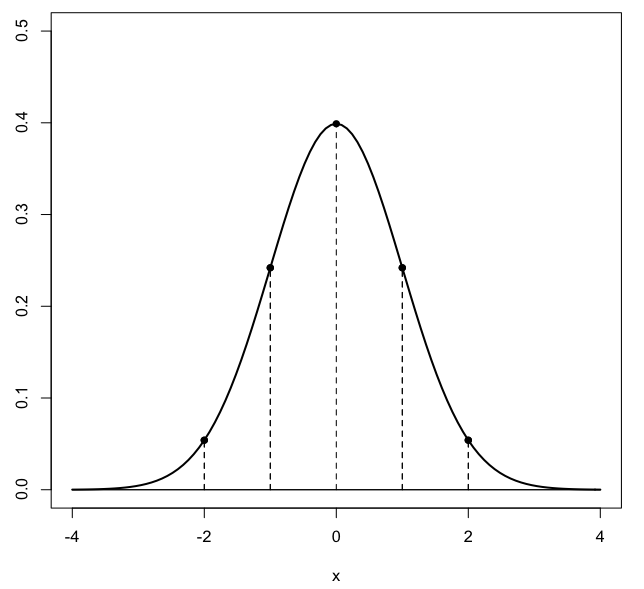
\includegraphics [scale=0.4] {gauss3.png} \end{center}

\begin{document}
\maketitle
\Large
\noindent
This is a derivation of Kepler's laws from a book I found on the web for Fitzpatrick's course on Mechanics.

\section{}
He starts by establishing unit vectors in polar coordinates as $\mathbf{e_r}$ and $\mathbf{e_{\theta}}$ and then parametrically
\[ \mathbf{e_r} =  \ \langle \cos \theta, \sin \theta \rangle \]
\[ \mathbf{e_{\theta}} =  \ \langle -\sin \theta, \cos \theta \rangle \]
\[ \mathbf{e_{\theta}} \perp \mathbf{e_r} \]
So
\[ \dot{\mathbf{e}}_\mathbf{r} = \dot{\theta} \mathbf{e_{\theta}} \]
\[ \dot{\mathbf{e}}_\mathbf{\theta} = -\dot{\theta} \mathbf{e_{r}} \]
Writing the position vector as
\[ \mathbf{r} = r \ \mathbf{e_r}  \]
\[ \mathbf{v} = \dot{\mathbf{r}} = \dot{r}\mathbf{e_r} + r \dot{\mathbf{e}}_\mathbf{r} =\dot{r}\mathbf{e_r} + r \dot{\theta} \mathbf{e_{\theta}} \]
For the acceleration
\[ \mathbf{a} = \dot{\mathbf{v}} = \ddot{\mathbf{r}} = \frac{d}{dt} \ (\dot{r}\mathbf{e_r} + r \dot{\theta} \mathbf{e_{\theta}}) \]
 \[ = \ddot{r}\mathbf{e_r} + \dot{r}\dot{\mathbf{e}}_\mathbf{r} + \dot{r} \dot{\theta} \mathbf{e_{\theta}} + r \ddot{\theta} \mathbf{e_{\theta}} + r \dot{\theta}  \dot{\mathbf{e}}_\mathbf{\theta}\]
\[ = \ddot{r}\mathbf{e_r} + \dot{r}\dot{\theta} \mathbf{e_{\theta}} + \dot{r} \dot{\theta} \mathbf{e_{\theta}} + r \ddot{\theta} \mathbf{e_{\theta}} - r \dot{\theta}^2  \mathbf{e}_\mathbf{r}\]
\[ = (\ddot{r} - r \dot{\theta}^2)  \mathbf{e}_\mathbf{r} + (2\dot{r} \dot{\theta} + r \ddot{\theta}) \mathbf{e_{\theta}}  \]
As before we recognize the coefficient for $\mathbf{e_{\theta}}$ as
\[ \frac{1}{r} \frac{d}{dt} (r^2\dot{\theta}) = \frac{1}{r}(2r \dot{r} \dot{\theta} + r^2\ddot{\theta})  \]
and this term is also equal to zero because the acceleration is all radial and so the term in parentheses must be zero and so
\[ 2 r \dot{r} \dot{\theta} + r\ddot{\theta} =  0 \]
if we integrate
\[ \int 2 r \dot{r} \dot{\theta} + r\ddot{\theta} = r^2 \dot{\theta} =  h \]
where $h$ is a constant.

The physical interpretation comes from angular momentum, which is defined as
\[ \mathbf{l} = m \mathbf{r} \times \dot{\mathbf{r}} \]
\[ = m (r \mathbf{e}_\mathbf{r} \times (\dot{r}\mathbf{e_r} + r \dot{\theta} \mathbf{e_{\theta}}) \]
\[ = mr^2  \dot{\theta} \ \hat{\mathbf{k}} \]
That is,
\[ mh \ = | \mathbf{l} | \]
At this point he goes through the standard analysis to obtain that the area swept out in a small time $\delta A/\delta t = h/2$.  I think we can skip this part.

\section{}
This derivation has an unusual approach to using the information from the inverse square law.  Define a new radial variable, the inverse of $r$
\[ r= \frac{1}{u} \]
Differentiate with respect to time
\[ \dot{r} = - \frac{\dot{u}}{u^2} \]
obviously.  But what is $\dot{u}$?
\[ \dot{u}= \frac{du}{dt} =  \frac{du}{d\theta} \frac{d\theta}{dt} =  \dot{\theta} \ \frac{du}{d\theta} \]
So
\[ \dot{r}= -\frac{1}{u^2} \dot{u} =  -\frac{\dot{\theta}}{u^2} \frac{du}{d\theta} \]
Recall $r^2 \dot{\theta} = \dot{\theta}/u^2 = h$ so
\[ = -h \ \frac{du}{d \theta}\]
Differentiate again with respect to time
\[ \ddot{r} = -h \frac{d}{dt} \ (\frac{du}{d \theta}) = -h \dot{\theta} \ \frac{d^2 u}{d\theta^2} \]
but $\dot{\theta} = hu^2$ so
\[ = - h^2 u^2 \  \frac{d^2 u}{d\theta^2} \]
Now, go back to our previous expression for the acceleration, it is
\[  - \frac{GM}{r^2}  =  \ddot{r} - r \dot{\theta}^2 \]
Plug in for $\ddot{r}$ and multiply everything by $-1$:
\[ \frac{GM}{r^2}  = h^2 u^2 \  \frac{d^2 u}{d\theta^2} + r \dot{\theta}^2 \]
Rearrange ($ru=1$):
\[ \frac{GM}{h^2}  =  \frac{d^2 u}{d\theta^2} + \frac{r^3}{h^2} \dot{\theta}^2 \]
but $h = r^2 \dot{\theta}$ and $h^2 = r^4 \dot{\theta}^2$ so
\[ \frac{GM}{h^2}  =  \frac{d^2 u}{d\theta^2} + \frac{1}{r}  \]
\[ \frac{GM}{h^2}  =  \frac{d^2 u}{d\theta^2} + u \]
How about that?  Now we have a basic differential equation in $u$

We guess the solution has, say $\cos \theta$ and constants $A$ and $C$.
\[ u = A \cos \theta + C \]
because
\[ \frac{d^2 u}{d\theta^2} = -A \cos \theta  \]
So
\[ C = \frac{GM}{h^2} \]
\[ u = A \cos \theta + \frac{GM}{h^2} \]
Technically, we should have $\theta_0$ in the solution, but we can just set that equal to zero, since we don't care about where we start.  Go back to $r$
\[ 1 = r(A \cos \theta + \frac{GM}{h^2}) \]
\[  \frac{h^2}{GM} = r(A \frac{h^2}{GM} + A \cos \theta) \]
Define 
\[ e = A = \frac{GM}{h^2} \]
so now we have
\[ \frac{h^2}{GM} = r(1 + e \cos \theta) \]
which is exactly what we had with Varberg.

\end{document}  